\chapter{Modularisierung} \label{cha:modularisierung}

% \section{Modularisierung} \label{sec:modularisierung}
  Modularisierungsansätze finden sich so gut wie in jeder Software wieder, da es sich um ein grundlegendes Prinzip für die Beherrschung eines Systems handelt. Gerade in der Java-Welt wird seit jeher das Ideal von lose gekoppelten Systemen verfolgt, denn diese generieren die Struktur in großen Softwareprojekten, indem das Gesamtprodukt in kleine, praktische Bestandteile zerlegt wird. \bigbreak
  
  Die Entwicklung von kleinen Projekten mit einer übersichtlichen Codebasis ist einfach zu überblicken und braucht keine strukturelle Unterstützung, um den Entwickler Architektur und Funktion darzustellen. Dennoch ist die Zukunft eines Projekts nicht immer eindeutig und kann mit der Zeit an Größe und Komplexität gewinnen. Mit der Größe des Projektes, wächst der Geschäftskontext und damit die Zahl der beteiligten Personen. Diese repräsentieren verzwickte Wünsche und Ziele, die an einer Stelle im Projekt nicht sauber umsetzbar sind. Infolge dessen ist die richtige Aufstellung eines Projektes von Grund auf eine zukunftssichere Entscheidung.\bigbreak 

  Ohne die Modularisierung werden Änderungen an großen Projekten mühselig und mit unerwarteten Nebeneffekten umgesetzt. Sowohl das Bauen und Ausrollen des Projekts als auch der Betrieb der Applikation ist eine lange und aufwendige Aufgabe, die mit jedem kleinen Fehler die komplett Applikation Neustarten lässt oder das Ausrollen unterbricht. Somit können kleine Fehler das ganze Produkt aus dem Gleichgewicht bringen. Aus diesem Grund sollen Module diese Probleme adressieren und die Applikation in autonome, kleine Einheiten aufteilen, die unabhängig voneinander ihre Funktionalität anbieten.

  % Moduleigenschaften 
  \section{Ziele der Modularisierung} \label{sec:ZdM}
    Die Modularisierung beschäftigt sich mit der Aufteilung eines Systems in Module, die Komplexität verringern, indem die einzelnen Module getrennt voneinander betrachtet und verstanden werden. Dies wiederum unterstützt die Wartbarkeit der einzelnen Module. Darüber hinaus vereinfachen die von der Modularität geforderte Schnittstellen Spezifizierung die Kommunikation zwischen den Modulen und fördert damit die Erweiterbarkeit des Systems. Da die Module austauschbar sind und unabhängig voneinander betrieben werden können, eröffnen sich neue Möglichkeiten der Softwareentwicklung. Wie zum Beispiel die Erstellung verschiedenen Varianten der Umsetzung, durch die Rekombination existierender Module, ohne die ganze Applikation zu in Betracht zu ziehen.\cite{javaMod9,java9modRevealed,explorJava9}\bigbreak

    Um die Aufgabe des Java Modularisierung zu verstehen, bedarf es einer Aufstellung von Zielen und Qualitäten, denen sich die Modularisierung stellt. Für JPMS sind diese eindeutig in der \textit{JSR 376} \cite{jmsOracle,java9modRevealed} beschrieben und spezifizieren die Folgenden Qualitäten.

    \subsubsection{Kapselung}
      Die Kapselung beschreibt ein Kontrollmechanismus, der die interne Struktur eines Moduls verwaltet. Demzufolge hat das Modul die komplette Kontrolle über ihre interne Struktur und kennt die Zugriffsrechte ihrer Bestandsteile, indem das Modul die Zugriffsrechte ihrer inneren Struktur explizit deklariert.

    \subsubsection{Interoperabilität}
      Die Interoperabilität beschreibt die Kommunikationsfähigkeit der Software mit anderen diversen Systemen, unabhängig von ihrer Sprache oder Plattform, mit der diese betrieben wird. Darum bieten Module Schnittstellen an, mit denen sie Dienste anbieten und anfordern können.

    \subsubsection{Zusammensetzbarkeit}
      Aus der Interoperabilität geht die Zusammensetzbarkeit hervor.  Diese Steht für die Wiederverwendbarkeit der in sich abgeschlossenen Module für unterschiedliche Zwecke in unterschiedlichen Systemen, indem man diese auf bestimmte Art und Weise kombiniert. 

    \subsubsection{Erweiterbarkeit}
     Die Erweiterbarkeit hilft den modularen und zusammengesetzten Systems ihre Funktionalität zu skalieren, indem die Software durch individuelle Einheiten ergänzt werden kann. 

    \subsubsection{Autonomie}
      Mit der Autonomie werden unnötige Abhängigkeiten aufgelöst und nur die nötige Funktionalität für die entsprechende Aufgabe in einem Modul abgelegt. Somit können einzelne Module im Betrieb auch dann bleiben, wenn Teile des Systems nicht reagieren.

  % Modulaufbau 
  \section{Modulstruktur}
      Die zuvor aufgeführten Ziele der Modularisierung liefern bereits eine Vorstellung der Modulanforderungen.
        \begin{figure}[h!] 
        \centering
        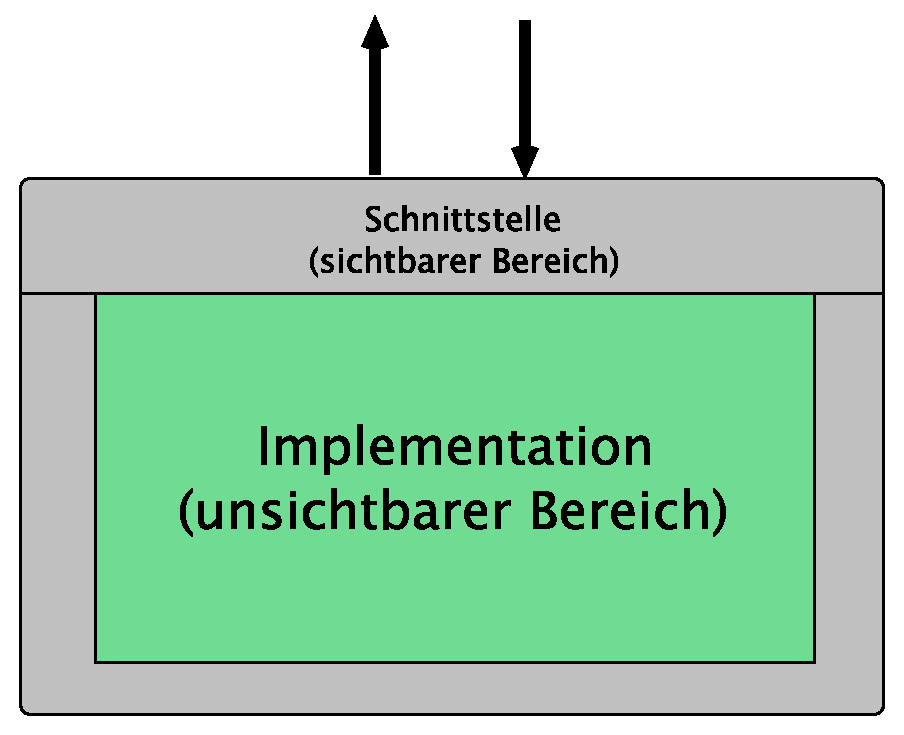
\includegraphics[width=0.4\textwidth]{material/images/simple-module.pdf}
        \caption{Simple Modulstruktur \cite{modulMitJava9}}
        \label{fig:simple-module}
      \end{figure}
    Primär erfüllt ein Modul einen abgeschlossenen Aufgabenbereich und beinhaltet die dafür nötigen öffentlichen sowie privaten Operationen und Datenfelder. Die Kommunikation eines Moduls mit anderen Modulen und der Außenwelt erfolgt über eindeutig spezifizierte Schnittstellen.\newline
    Somit dient das Modul als ein Behälter für Objekte, der aus einem unsichtbaren und einem sichtbaren Bereich besteht. Der sichtbare Bereich ist die Schnittstelle des Moduls und ist die Aufzählung derer Objekte, die das Modul nach außen hin zur Verfügung stellt. Der Zugriff auf diese erfolgt über definierte Operationen in der Modulschnittstelle. Der unsichtbare Teil beherbergt die eigentliche Implementierung, also die umgesetzten Operationen und Daten. Unter diesen Umständen reduziert sich die Komplexität des Moduls für den Nutzer von der gesamten Implementation auf die Schnittstellen. \cite{javaMod9,java9modRevealed,explorJava9,modulMitJava9}

      \begin{figure}[h!]
        \centering
        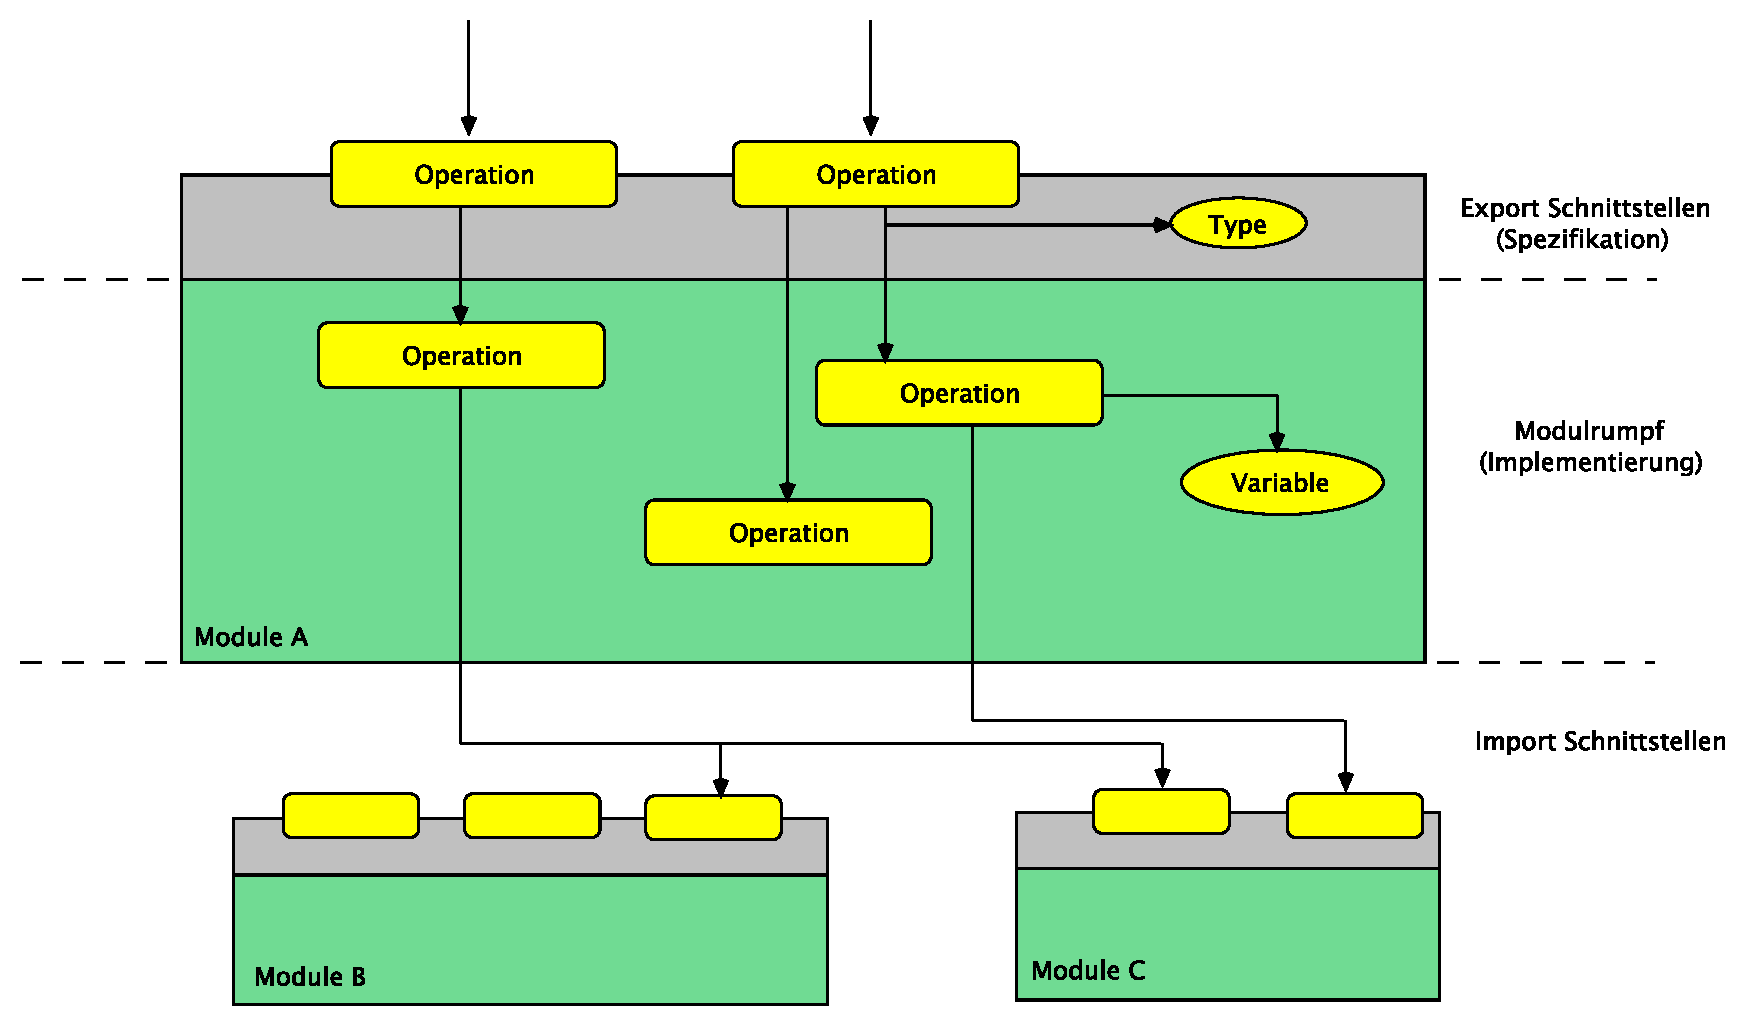
\includegraphics[width=\textwidth]{material/images/Module-workflow.pdf}
        \caption{Schematischer Aufbau eines Moduls \cite{modulMitJava9}}
        \label{fig:mw}
      \end{figure} 

    In der Abbildung \ref{fig:mw} wird die interne Struktur sowie entsprechenden Verbindungen eines Moduls genau betrachtet. Zu sehen sind drei Module, die ihre Dienste mit dem \textit{exports} Schlüssel über die Schnittstellen anbieten und diese bei Bedarf mit anderen Modulen kombinieren können, indem weitere Funktionalität durch den \textit{requires} Schlüssel von zusätzlichen Modulen angefordert wird. Die interne Umsetzung der Funktionalität bleibt jedoch verborgen und kann Modulübergreifend nicht nachverfolgt werden. 

  % Moduldefenition schlussatz als zusammenfassung 
  \section{Moduleigenschaften} \label{sec:ME}

    \textbf{Modul Definition: } \textit {Ein Modul ist eine Sammlung von Algorithmen und Daten bzw. Datenstrukturen zur Bearbeitung einer in sich abgeschlossenen Aufgabe. Die Verwendung des Moduls (d.h. seine Integration in ein Programm-System) erfordert keine Kenntnis seines inneren Aufbaus und der konkreten Realisierung der gekapselten Algorithmen und Daten(-strukturen). Seine Korrektheit ist ohne Kenntnis seiner Einbettung in ein bestimmtes Programmsystem nachprüfbar.} \cite{rechenberg2006informatik}\bigbreak 

    Aus dieser Definition können folgende Eigenschaften abgeleitet werden, die ein Software-Modul beschreiben:

    \begin{itemize}
      \item Zusammenfassung von Operationen und Daten zur Realisierung einer in sich abgeschlossenen Aufgabe 
      \item Kommunikation mit der Außenwelt nur über eine eindeutig spezifizierte Schnittstelle 
      \item Nutzung des Moduls möglich ohne Kenntnis des inneren Ablaufs 
      \item Die Struktur jedes Moduls sollte einfach genug sein, um vollständig verstanden zu werden.
      \item Anpassungen eines Moduls sollte ohne Kenntnis der Implementierung sowie ohne Einfluss auf das Verhalten anderer Module durchführbar sein.
      \item Korrektheit des Moduls durch Tests nachprüfbar ohne Kenntnis seiner Einbettung
      \item Wiederverwendbarkeit der Funktionalität im anderen Kontext
    \end{itemize}

  % Wie modelliert man Module  
  \section{Modulentwurfskriterien} \label{sec:MEK}
    % Einleitung
    Nachdem die Struktur des Moduls klar bestimmt wurde, muss die Umsetzung einer Applikation mit Modulen auf Qualitätsmerkmale abgeglichen werden. Da die Aufteilung eines Entwurfsproblems in kleinere Teilprobleme nicht selbstverständlich ist, kann diese mit verschieden Techniken und auf diverse Weise umgesetzt werden und bietet daher keine Garantie eines sauberen Entwurfs. Die Kunst Funktionalität in einem einzelnen Modul zu kapseln und diese mit geringer Abhängigkeit vom Restsystem betreiben zu können, kann mithilfe bestimmter Kriterien bewertet und angepasst werden. \cite{softModDes,softMdDes2,modulMitJava9,java9modRevealed,modulProgJava9}\bigbreak
    
    Bei der Modularisierung sind folgende Entwurfskriterien zu berücksichtigen: 
    \begin{itemize}
      \item Modulgeschlossenheit 
      \item Maximale Modulbindung 
      \item Minimale Modulkopplung 
      \item Minimale Schnittstelle 
      \item Modulanzahl 
      \item Modulgröße 
      \item Testbarkeit 
      \item Seiteneffektfreiheit 
      \item Importzahl 
      \item Modulhierarchie 
    \end{itemize}
    Mithilfe der \textit{Modulgeschlossenheit} wird die Abhängigkeit des Moduls von anderen Modulen reduziert und lässt diese separat bearbeiten und austauschen. Somit kapselt ein Modul eine bestimmte Funktionalität, die von Anfang bis zum Ende intern verarbeitet werden kann. Direkt daraus folgt im besten Fall eine \textit{maximale Bindung} oder starker Zusammenhang innerhalb eines Moduls, indem die internen Komponenten bestens mit einander verzahnt sind und sich gemeinsam mit einer gezielten Aufgabe beschäftigen. In der Konsequenz entsteht ein eingeschränkter Wartungsraum für Entwickler, die sich mit der entsprechenden Funktion beschäftigen. Um die Bindung der Komponenten innerhalb eines Moduls zu messen, können die Abhängigkeiten in verschieden Kategorien eingeteilt werden: logisch, zeitlich, prozedural, sequentiell, informal und funktional.

    \begin{figure}[h]
      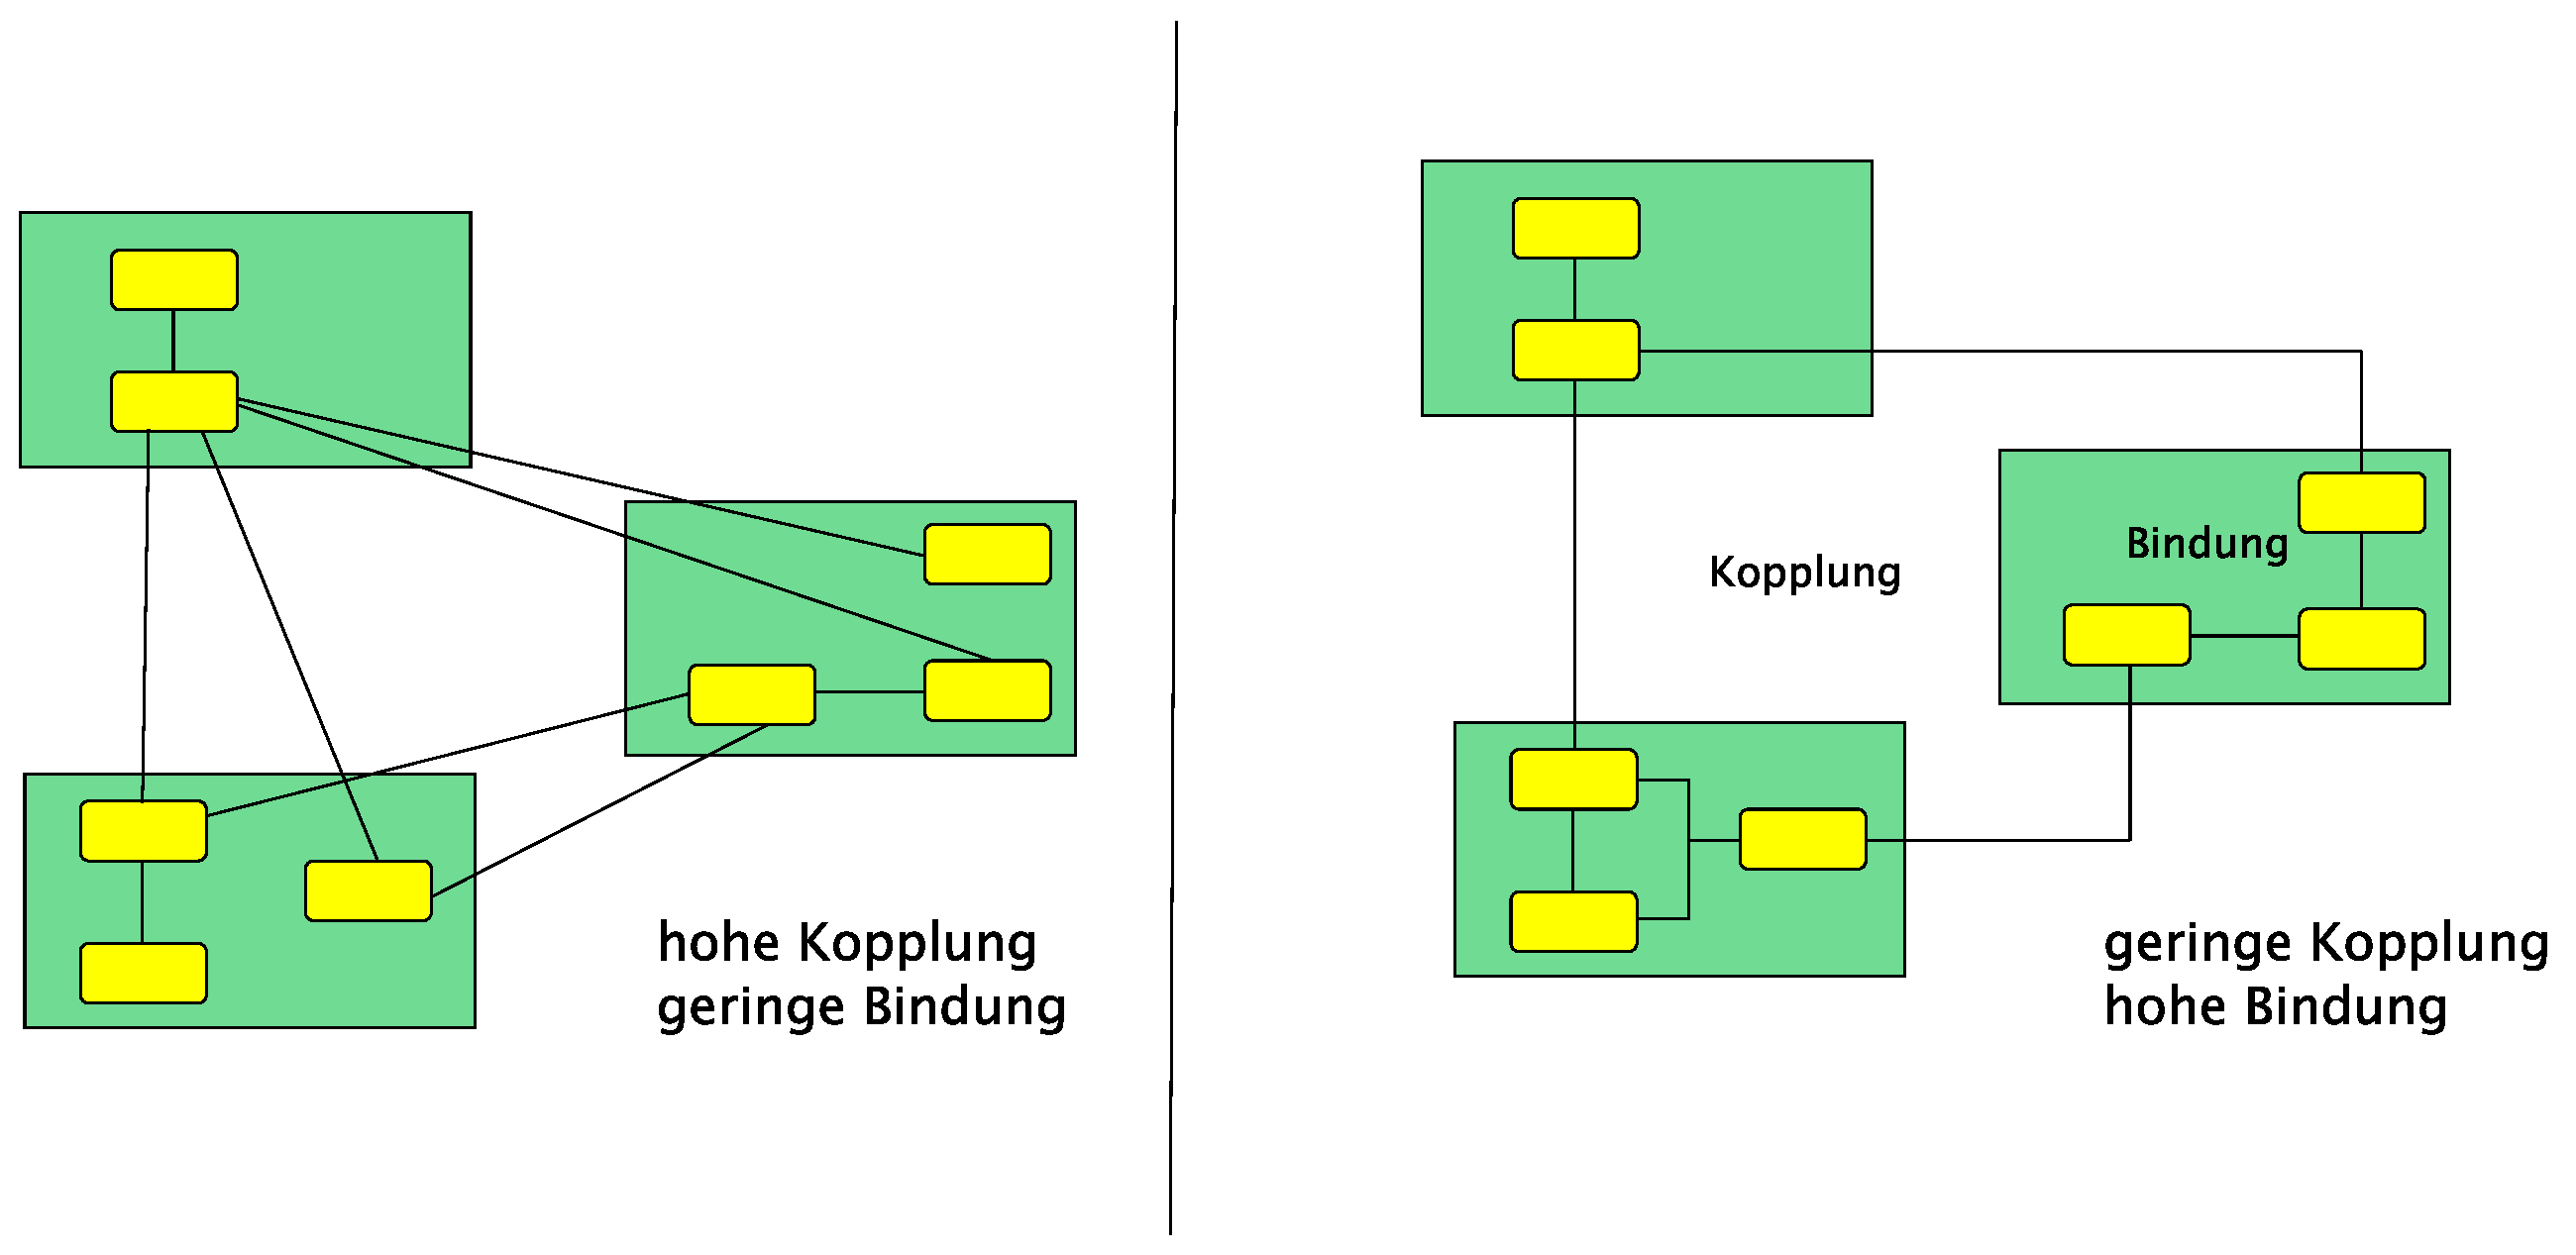
\includegraphics[width=\textwidth]{material/images/kopplung.pdf}
      \caption{Modulbindung und Modulkopplung \cite{modulMitJava9}}
      \label{fig:kopplung}
    \end{figure}

    Komplementär zu der \textit{maximalen Bindung} beschreibt die \textit{minimale Kopplung} die Anzahl der Verbindung zwischen den Modulen. Diese sollte natürlich klein gehalten werden, um die Abhängigkeit zu reduzieren. Die \textit{minimale Kopplung} hat somit einen direkten und positiven Einfluss auf die Anzahl der Schnittstellen, indem diese übersichtlich und eindeutig die Funktion des Moduls beschreiben. Andernfalls kann eine starke Kopplung die Komplexität heben und Fehler begünstigen, indem der Umfang an Daten, die zwischen den Modulen ausgetauscht werden, erhöht wird. Eine \textit{minimale Kopplung} ist ein guter Ansatz den unnötigen Datentransfer zu reduzieren, garantiert aber keine lose Kopplung von den umgebenen Modulen. Daher sollte der Begriff \textit{Seiteneffektfrei} eingeführt werden. Dieser beschreibt den Einfluss eines Moduls auf seine Umgebung, indem das Modul Unverzichtbar für die Gesamtfunktionalität wird und der Austausch die Anpassung verknüpfter Module nach sich zieht. Das ist öfters der Fall, wenn eine Aufgabe modulübergreifend gelöst werden muss und die Aufgabenkapslung für diesen Zweck aufgelöst wird.\cite{softModDes,softMdDes2,modulMitJava9,java9modRevealed,modulProgJava9}

    % Modularten wie Platform Explicit Modules, Application Explicit Modules, Automatic Modules, Open Modules, Unnamed Module 
  \section{Modularten} \label{Modularten}
    Das Modulsystem von Java unterscheidet die Module in fünf unterschiedliche Arten, diese richten sich nach der Aufgabe und ihrer Umsetzungsstruktur. Zum einen gibt es die JDK \textit{Plattform Module}, die die Kernfunktionalität der Java Laufzeitumgebung bieten und Pakete wie \textit{java.lang, java.io} und \textit{java.net} mit sich bringen. Andererseits gibt es die Benutzer konstruierten \textit{Applikationsmodule}, die durch eine explizite Komposition bestimmte Aufgaben erfüllen. Beide Modultypen beinhalten eine \textit{Modulbeschreibung}, die dessen Abhängigkeiten und Schnittstellen beschreibt. \newline
    Obwohl mit den vorher genannten \textit{expliziten Module} Softwaresystemen realisieren lassen, fehlt die Offenheit bestimmter Module oder ihrer Pakete für die Umsetzung der Reflection Bibliotheken, die dynamischen Zugriff auf unsere Pakete während der Laufzeit benötigen. Wie im Kapitel \ref{sec:refl} besprochen ist Reflection ein wichtiges Werkzeug in der Softwareentwicklung und wird in dem neuen Java Modulsystem unterstützt. Um Reflection in einem Modul zu aktivieren, reicht es lediglich das ganze Modul als \textit{open module} oder mithilfe des \textit{opens package.name} Schlüssels ein spezielles Paket des Moduls in der \textit{Modulbeschreibung} zu deklarieren. Damit hätte man ein für Reflection offenes Modul und könnte dessen öffentlichen sowie privaten Klassen dynamisch aus jedem Modul auf dem Modulpfad aufrufen. Da diese Module das Konzept der starken Kapselung aufgeben, werden diese zu einem besonderen Typen der \textit{offenen Module} zugeordnet. \cite{modulMitJava9,java9modRevealed,modulProgJava9,explorJava9}

    \begin{figure}[h]
      \centering
      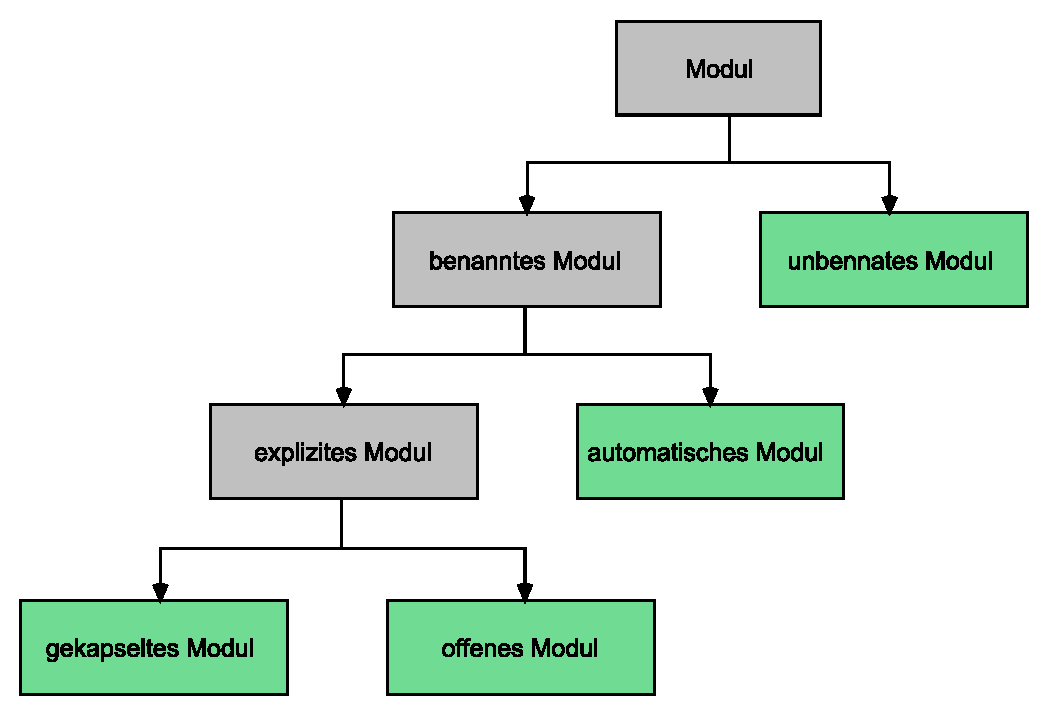
\includegraphics[width=0.7\textwidth]{material/images/module-tree.pdf}
      \caption{Modularten \cite{modulMitJava9}}
      \label{fig:modtree}
    \end{figure}

    Die nachfolgenden Modultypen sind Pseudo-Module, die für die Unterstützung der Abwärtskompatibilität eingeführt worden sind. 
    Dementsprechend sollen diese Module eine Brücke zwischen existierender Applikation und der modularisierten Architektur bilden.\bigbreak

    Das \textit{unbenannte Modul} beschreibt alle Klassen und JAR's, die sich parallel zu der Codebasis des Modulpfades auf dem Klassenpfad befinden. Das \textit{unbenannte Modul} beschreibt somit den Legacy-Teil der Codebasis, die noch migriert werden muss und es noch nicht tun kann. Daher wird mit der Bezeichnung \textit{unbenanntes Modul} eine Zugriffsbarriere zwischen der modularisierten und der legacy Architektur errichtet, die die \textit{expliziten Module} vom Zugriff auf den veralteten Klassenpfad abgrenzt. Denn dieses trägt keinen Namen und kann somit vom Entwickler nicht pragmatisch referenziert werden.\newline
    In Folge dessen entsteht eine asymmetrische Kommunikation zwischen den Architekturen. Die \textit{expliziten Module} arbeiten nur auf dem Modulpfad im neuen System und das \textit{unbenannte Module} darf zusätzlich zu den klassischen Klassenpfad auf den modernen Modulpfad zugreifen. Diese Umsetzung lässt eine inkrementelle Migration der Codebasis auf das Modulsystem zu und bleibt lauffähig, obwohl die Applikation eine interne Versionsdiskrepanz beinhaltet. \cite{modulMitJava9,java9modRevealed,modulProgJava9}

    \begin{figure}[h]
      \centering
      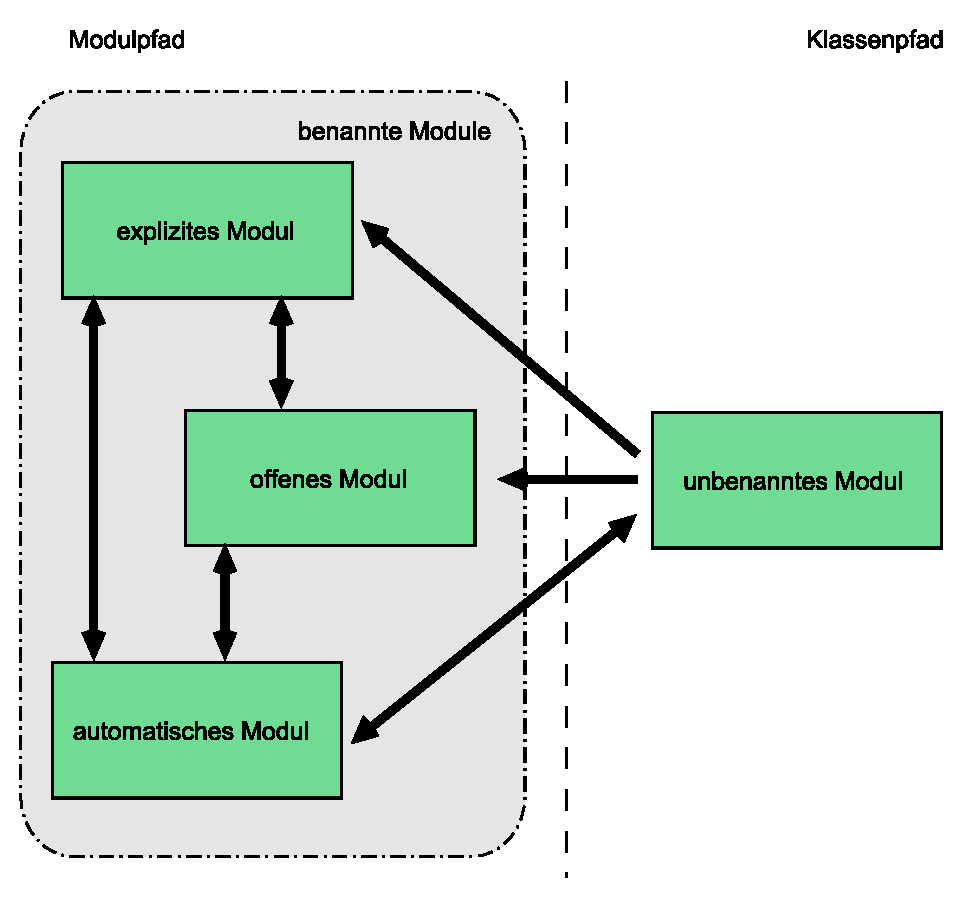
\includegraphics[width=0.7\textwidth]{material/images/module-access.pdf}
      \caption{Modulzugriffsrechte \cite{modulMitJava9}}
      \label{fig:modacc}
    \end{figure}

    Das letzte Modul beschreibt ein Modul mit speziellem Verhalt, das sich zwischen den Architekturen stellt und eine Brücke zwischen den Modulpfad und Klassenpfad errichtet. Die \textit{automatischen Module} beschreiben einen Migrationsansatz der bestehenden Bibliotheken, die vom Klassenpfad auf den Modulpfad verschoben werden und keine \textit{Modulbeschreibung} besitzen. Diese kriegen einen Modulnamen zugewiesen und können über diesen von den \textit{expliziten Modulen} aufgerufen werden. Somit übernimmt Java die Kopplung der \textit{automatischen Module} mit allen \textit{expliziten Modulen}, indem alle internen Pakete für die Nutzung offengelegt werden und alle Module auf dem Modulpfad für die Verwendung importiert werden. In der Folge ist eine Legacy-Bibliothek auf den Modulpfad funktionstüchtig und bietet eine ganz besondere Fähigkeit, nämlich die wechselseitige Kommunikation zwischen dem Modulpfad sowie dem Klassenpfad. Dank dieser Fähigkeit können Bibliotheken migriert werden und beide Architekturen zu gleich unterstützen. Dieses Verhalten fördert die Entwickler ihren Code für den Modulpfad zu entwickeln, da die nötigen Legacy-Bibliothek der Applikation in beiden Architekturen zugleich verfügbar ist.\newline 
    Dennoch schaffen die \textit{automatischen Module} zusätzliche Komplexität in die Architektur, indem alle Module mit diesem verbunden werden. Daraus folgt eine starke Kopplung und somit eine unübersichtliche, starke Abhängigkeit zwischen den Modulen.\cite{modulMitJava9,java9modRevealed,modulProgJava9}\bigbreak

    Nichtsdestotrotz bietet das automatische sowie das unbenannte Modul diverse Migrationsszenarien, die flexible Wege für die Modernisierung der Applikation anbieten. 

  \section{Modulkopplung} \label{sec:mod_kop}
    Die Einführung des Modulsystems in Java 9 integriert das Konzept der Aufteilung einer monolithischen Softwareumsetzung in übersichtliche mit einander sachlich verbunden Modulen. Diese Idee wird zuerst von Java selbst umgesetzt, um als Beispiel für den aufbauenden Code zu fungieren. In der praktischen Umsetzung formuliert Java die Modulbeschreibung mithilfe der \textit{module-info.java} Datei, die drei Kopplungstypen enthalten kann: die durch \textit{requires, exports} und \textit{opens} Deskriptoren beschrieben wird.

    \begin{figure}[h!]
      \centering
      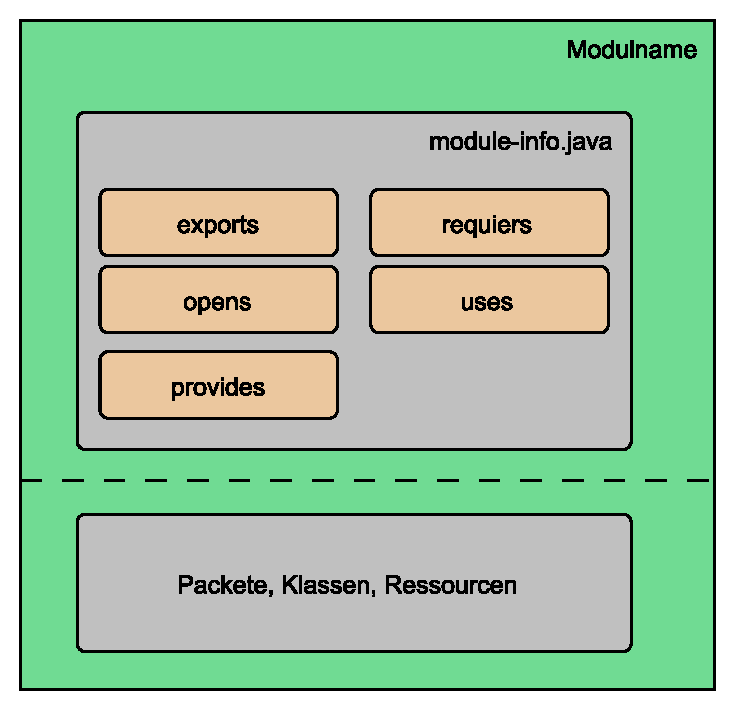
\includegraphics[width=0.5\textwidth]{material/images/module-info.pdf}
      \caption{Die Schnittstellenbeschreibung \textit{module-info.java}}
      \label{fig:module-info}
    \end{figure}

    Die in der Abbildung \ref{fig:module-info} dargestellten und vorher diskutierten Kopplungsarten, können die Zugriffsberechtigungen ferner einschränken. Diese können ihre Schnittstelle exklusiven Modulen öffnen, die fortan als eine transitive Verbindung weiterreichen und obendrein als eine optionale Abhängigkeit deklarieren. Die \textit{uses} und \textit{provides} Schlüssel beschreiben eine Serviceanfrage sowie einen Serviceangebot, die durch den \textit{Java ServiceLoader} mit einender verknüpft werden.\newline
    Der \textit{ServiceLoader} übernimmt in diesem Fall die Rolle des Registrierungsdienstes und vermittelt das Angebot und die Nachfrage nach Funktionalität innerhalb der Applikation. Das Konzept der Dienstregistrierung und der Dienstverwaltung geht über die Grundlagen hinaus und wird hier nicht weiter diskutiert, dessen ungeachtet ist es eine zusätzliche Möglichkeit die Modulkopplung zu minimieren. \cite{softModDes,modulMitJava9} \bigbreak

      \begin{figure}[h!]
      \centering
      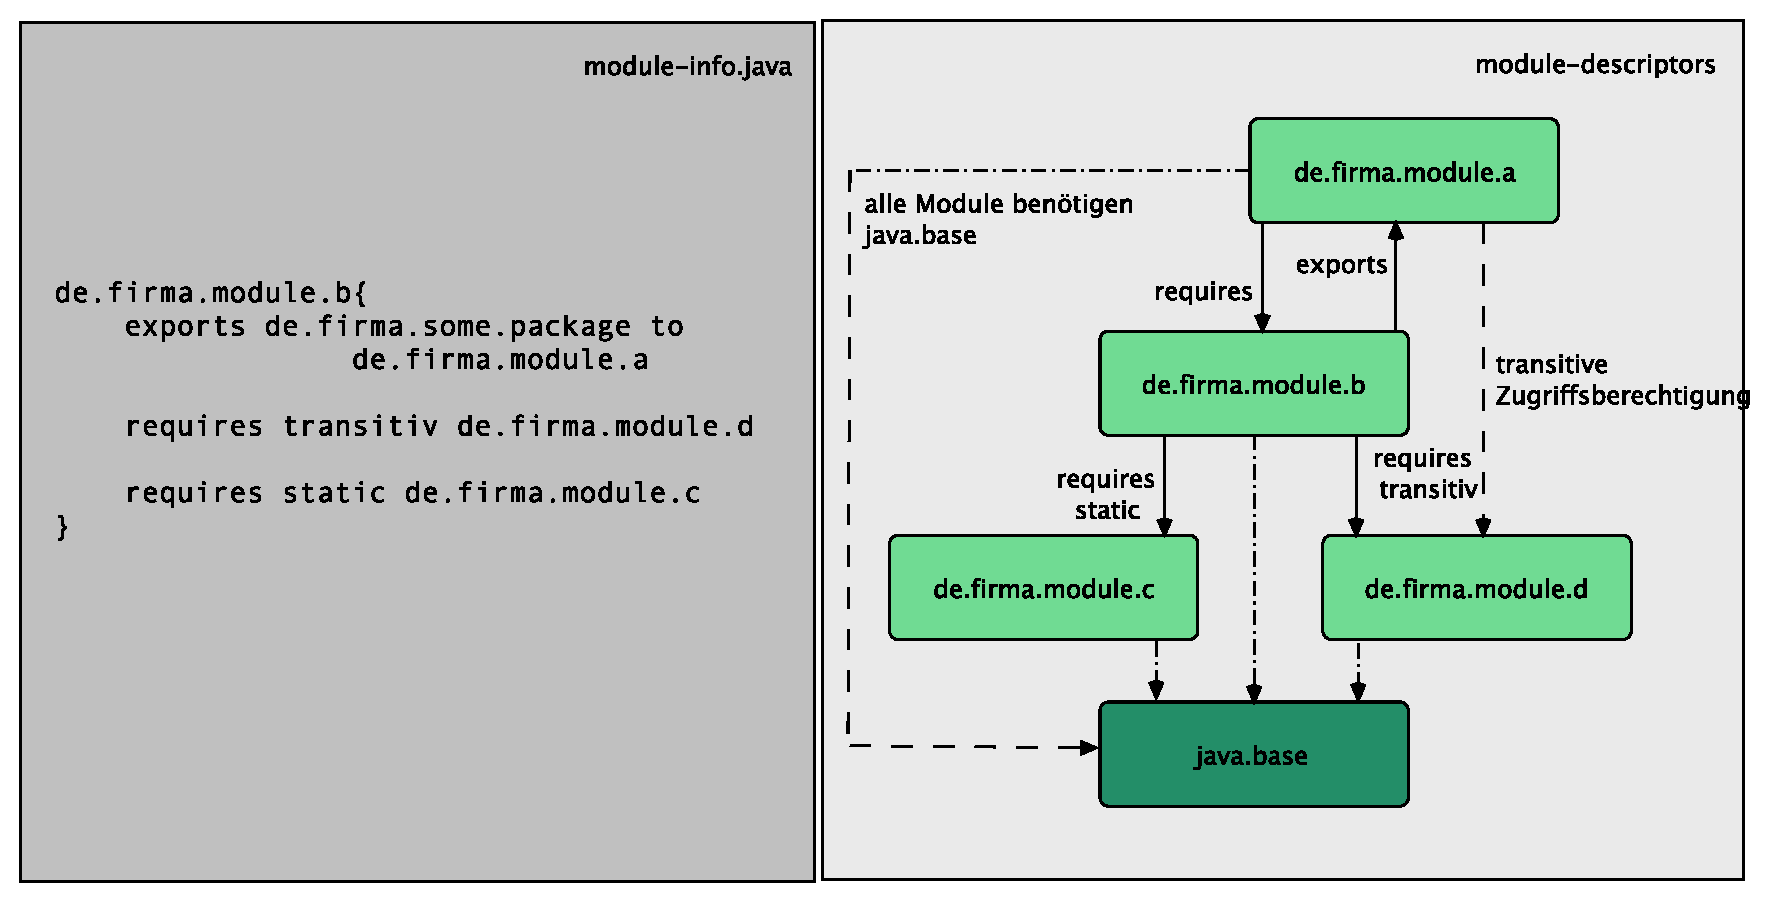
\includegraphics[width=\textwidth]{material/images/transitiv.pdf}
      \caption{Abwandlung der Kopplungsarten}
      \label{fig:abw-kopl}
  \end{figure}

    Im Folgenden werden die in der Abbildung \ref{fig:abw-kopl} dargestellten Möglichkeiten der Kopplungstypen gelistet. Zu beachten ist die Wechselbeziehung zwischen den Modulen, die Pakete anbieten und Module anfordern. \cite{jmsOracle}

    \begin{description}
      \item[requires]\hfill
      \newline \textit{requires} Modul
      \newline \textit{requires transitiv} Modul
      \newline \textit{requires static} Modul
      \newline \textit{requires transitiv static} Modul
      \item[exports]\hfill
      \newline \textit{exports} Packet
      \newline \textit{exports} Packet \textit{to} Modul-1, Modul-2
      \item[opens]\hfill
      \newline \textit{opens} Packet
      \newline \textit{opens} Packet \textit{to} Modul-1, Modul-2
      \item [uses]\hfill
      \newline \textit{uses} Service-Schnittstelle 
      \item[provides]\hfill
        \newline \textit{provides} Service-Schnittstelle \textit{with} Service-Impl-1, Service-Impl-2
  \end{description}


  Wie in der grafischen Darstellung \ref{fig:abw-kopl} abgebildet, handelt es sich bei den Kopplungstypen um Zugriffsrechte, die als ein offener Vertrag zwischen Modulen aufgestellt werden. Dementsprechend dienen die Kopplungsschlüssel nicht nur der Lesbarkeit und Autonomie, sondern erweitern die Prozedur des Klassenladens durch explizite Schnittstellen und Zugriffsberechtigungen.\cite{modulMitJava9}

  \section{Module Classloading} \label{sec:mod-cll}
    Im Abschnitt \ref{sec:nam} wurden Namensräume vorgestellt, die Klassen von einender trennen und diese als separate Software Komponenten behandeln, um die Sichtbarkeit der Codebasis gegenüber dem Restsystem abzugrenzen. Jedoch bring dieses Feature einen großen Aufwand mit sich, denn sofern die Applikation eine große Anzahl an Bibliotheken benutzt und jedes davon auf einem eigenen Classloader betreiben möchte, wächst der Wartungsaufwand mit der Anzahl der Bibliotheken.\newline
    Mithilfe der Module und dessem neuem Ansatz der internen Kapselung, soll dieses Problem adressiert werden, indem separate Zugriffsräume für jedes Modul innerhalb eines Classloaders definiert werden, die sicherstellen, dass die interne Struktur eines Moduls während der Laufzeit nicht kompromittiert werden kann.\newline
    Für die Garantie der Modulkapselung, wird das im Abschnitt \ref{sec:cls} vorgestellte \textit{Java Classloader System} nicht ersetzt, sondern mit zusätzlichen Kontrollen versehen, die strikt nach deklarierten Modulbeschreibung Zugriff gewährleistet. Im Falle der Nichteinhaltung der Zugriffsrechte zwischen den Modulen wirft der Classloader neue Fehlermeldungen wie die \textit{IllegalAccessException} oder die \textit{IllegalAccessError}. Somit bleibt die ehemalige Classloader Hierarchie erhalten, die an das Modulsystem von Java angepasst worden ist. \cite{classLoadingOracle, modulMitJava9}\bigbreak

    Um die neuen Kontrollmechanismen im Java Kern zu verankern, wurde der die \textit{rt.jar}, die für die Ausführung von Java Code zuständig ist, auf Module mit expliziten Aufgabenbereichen aufgeteilt. Wie in der Abbildung \ref{fig:jdk} abgebildet, beschäftigt sich das aktualisierte \textit{Classloader System} mit dem Laden bestimmter Module, die in Gültigkeitsbereiche fragmentiert sind. Diese nutzen immer noch das Delegierungsmodell \ref{sec:dm} und delegieren jede Anfrage zuerst an den Wurzel-Classloader. Mit dem Modulsystem von Java wurde dieses Verfahren durch zwei Sicherheitsverfahren erweitert. Das erste Verfahren löst eins der größten Schwierigkeiten der Java Entwickelung, nämlich das Management der Abhängigkeiten eines Systems. Diese Herausforderung wird als \textit{Jar-Hell} bezeichnet und beschreibt eine komplexe Applikation, die eine lange Liste an genutzten Drittanbieter Bibliotheken benötigt. Das Problem taucht auf, da der Java Code den Klassenpfad nicht kontrolliert und annehmen muss, dass alle benötigten Bibliotheken auf den Klassenpfad vorhanden sind. Die Lokal eingerichtete Maschine oder Entwicklungsumgebung kann das Management verwalten, jedoch kann diese nicht garantieren, dass die Software in einer anderen Umgebung funktionsfähig bleibt.\newline
    Dieser Anforderung hat sich das Modulsystem von Java gestellt und bietet die phasenübergreifende Wiedergabetreue auf allen Systemen, indem jedes Modul eine Voraussetzung deklariert, die der Modulpfad erfüllen muss, bevor die Applikation ihre Arbeit beginnt. Somit wird das gleiche Verhalten sowie Fehlerprüfungen in der Kompilierungs- und Ausführungsphase erreicht.\newline
    Das zweite Verfahren garantiert die Einhaltung der Nutzungsrechte einer Bibliothek, indem die Nutzung einer Bibliothek über klar definierte Schnittstellen geschieht und unterbindet somit den impliziten Zugriff auf den Inhalt innerhalb eines Namensraums. Beide Verfahren berufen sich auf die \textit{module-info.java} Konfigurationsdatei, die in sich die benötigte Information verankert. \bigbreak

    Um die Klassen aus dem Modulpfad zu laden, wurde das \textit{Classloader Systems} an den Modulpfad angepasst und lädt jetzt Module, die nach Sicherheitsberechtigungen bestimmten \textit{Classloader}zugewiesen werden. Der \textit{Bootstrap Classloader} ist der \textit{Classloader} der JVM und genießt alle Sicherheitsprivilegien. Dieser lädt die \textit{Core Java-SE} und \textit{JDK-Module}, wie \textit{java.base} und \textit{java.logging}. Der Extension Classloader wurde von dem Plattform Classloader ersetzt und lädt jetzt die \textit{Plattform Java-SE} Module, wie zum Beispiel die \textit{java.sql}, oder die \textit{java.xml.ws} Bibliotheken. Und zuletzt bleibt der Applikation Classloader, der unsere Applikationsmodule auf dem Modulpfad verwaltet. \cite{classLoadingOracle,modulMitJava9,java9modRevealed}

  \section{Module Loading} \label{sec:module_Loading}
   Obwohl das Klassenlader-Konzept von Java seine Gültigkeit behält, gibt es mit dem Einzug der modularisierten Plattform einige Änderungen. Mit dem Modulsystem von Java wir ein neues Konzept der Modulschichten eingeführt, das für das Laden von Java Code während der Laufzeit verantwortlich ist. Die Modulschichten validieren, kapseln und laden bestimmte Modulgruppen, die während der Laufzeit einer Applikation integriert werden können. Somit erweitern die Schichten das bestehende Klassenlader-Konzept durch erweiterte API's für die Verwaltung vom dynamischen Code und erzwingen zusätzlich die Korrektheit der Modulabhängigkeiten die dem System hinzugefügt werden. 

   \subsubsection{Module Graph}\label{sub:module_graph}
   \subsection{Module Layer} \label{sub:module_layer}


- Classlaoder System bleibt 
-  Es gibt zusätzliche Erweiterungsmöglichkeiten 
- beim Start wird eine bootschicht erzeugt 

\section{JDK Modulsystem} \label{sec:modular_java_base}
  Um die Aufgestellten Regeln und Konzepte des entworfenen Modulsystems in Java zu integrieren, muss die Java Plattform diese selbst als Vorreiter erfüllen. \bigbreak
  Demnach wurde die Laufzeitumgebung (\textit{Run-Time}), die aus der \textit{rt.jar} besteht, auf Module aufgeteilt und mit einander über Kommunikationsregeln und Schnittstellen verknüpft. Das Ergebnis der modularisierten \textit{rt.jar} ergab 70 Module, die sich gegenseitig ergänzen. \newline
  In der Konsequenz ist eine kleine Applikation, die sich nur an dem \textit{base} Modul bedient, mit einem Speicherbedarf von 16 MB umsetzbar. Im Gegensatz dazu müssten für ein paar Zeilen Code in der 8 Version von Java, 160 MB der \textit{rt.jar} in die Laufzeitumgebung miteinbezogen werden, um den Laufzeitanforderungen zu entsprechenden.\bigbreak
  \begin{figure}[h!]
   \centering
   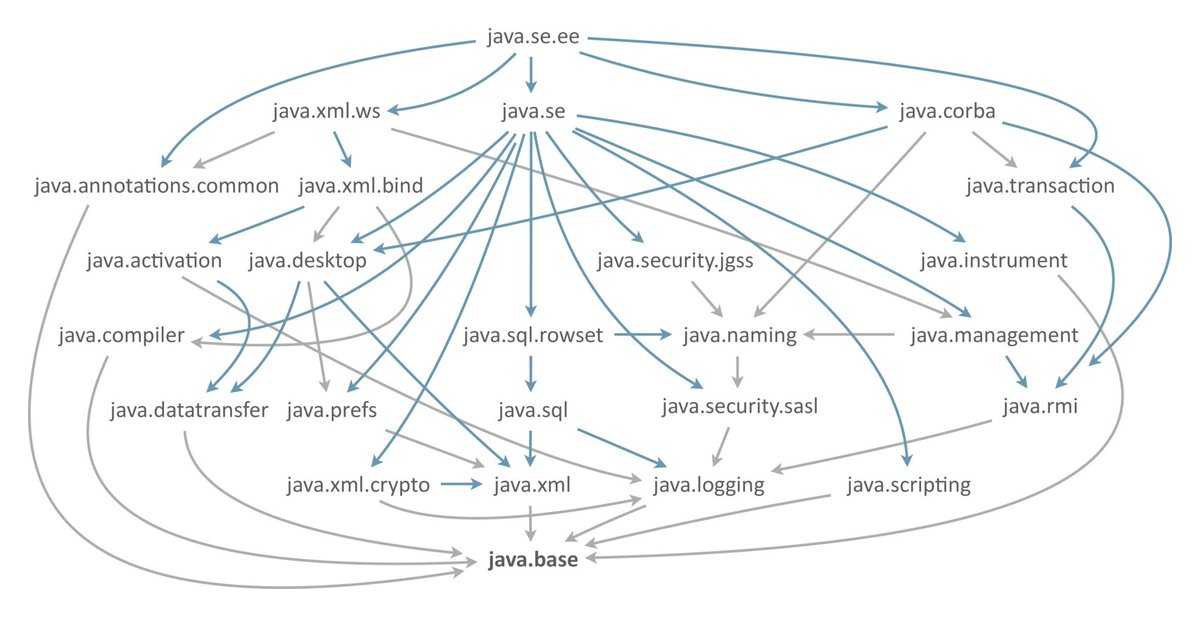
\includegraphics[width=\textwidth]{material/images/moduleGraph.jpg}
   \caption{Modularisierte \textit{rt.jar} Laufzeitumgebung \cite{modGraph}}
   \label{fig:jdk}
  \end{figure}
  Obwohl das Modulsystem viele Neuerungen und Aufwertungen der Java Plattform mit sich brachte, sind nicht alle Wünsche erfüllt worden. Wie zum Beispiel das Nutzen gleichnamiger Bibliotheken mit unterschiedlicher Versionsnummer auf demselben Modulpfad.\newline
  Nichtsdestotrotz gibt es Ansätze, die es erlauben eine Versionsnummer in einem Modul zu verankern und somit existiert die Wahrscheinlichkeit, dass dieser Fähigkeit in der Zukunft nachgerüstet wird. 
 

